\documentclass[a4j]{ujarticle}
\usepackage[dvipdfmx]{graphicx}
\usepackage{url}
\usepackage{bbding}
\usepackage{lscape}


\title{ミーティング資料}
\author{安達智哉\\to-adachi@ist.osaka-u.ac.jp}
\date{平成30年12月13日}

\begin{document}
\maketitle

\section{vEPCを想定した負荷分散モデルの検討}
3GPP標準に基づく負荷分散方式を、他方式と比較するような研究を行おうと考えている。他方式として具体的にはvEPC間の負荷分散方式を想定している。vEPC想定したネットワーク構成のモデル案を以下の図\ref{vEPC}に示す。このモデルでは、ネットワークに分散しているvEPCの中から適切なvEPCを選択し、それを経由するようにシグナリングを設定する。この仕組みにより負荷分散が可能である。このモデルの評価を行う上で大切なことは、vEPC間のState同期によるオーバヘッドを考慮することである。実際、文献\cite{PerformanceComparisonofStateSynchronizationTechniquesinaDistributedLTEEPC}によると、MME間のState同期のオーバヘッドより、最大71\%の性能低下が発生すると結論づけている。また、Stateの同期頻度にも複数の実装があると述べており、メッセージごとに同期を行う方法とセッションごとに同期を行う方法でオーバヘッドが変化すると述べている。そのため、評価指標の一つとして、vEPC間のState同期のオーバヘッドを取り入れようと考えている。


また、vEPCを用いたネットワーク構成として、データプレーンをSDNを用いて制御するモデルも想定することができる。図\ref{vEPC_SDN}には、図\ref{vEPC_model}に示したモデルにSDNを適用したモデルである。vEPCにSDNコントローラが存在し、SDNスイッチに指示することでデータプレーンを制御する。この際、SDNコントローラにはSGW-CおよびPGW-Cの機能を持たせる必要があり、SDNスイッチは、S/PGWの機能を持つように拡張する必要がある。図\ref{vEPC}と比較すると、こちらの方式の方が、データプレーンの経路を短くできることが分かる。また、SDNの制御により、帯域の使用率に応じて、データプレーンの経路を変化させることも可能である。そのため、vEPCのCPU使用率に基づいた負荷分散と同時に、リンク帯域の使用率に応じた負荷分散が可能になると考えられる。

\begin{figure}[p]
	\centering
		\begin{subfigure}{1.0\textwidth}
		\centering
			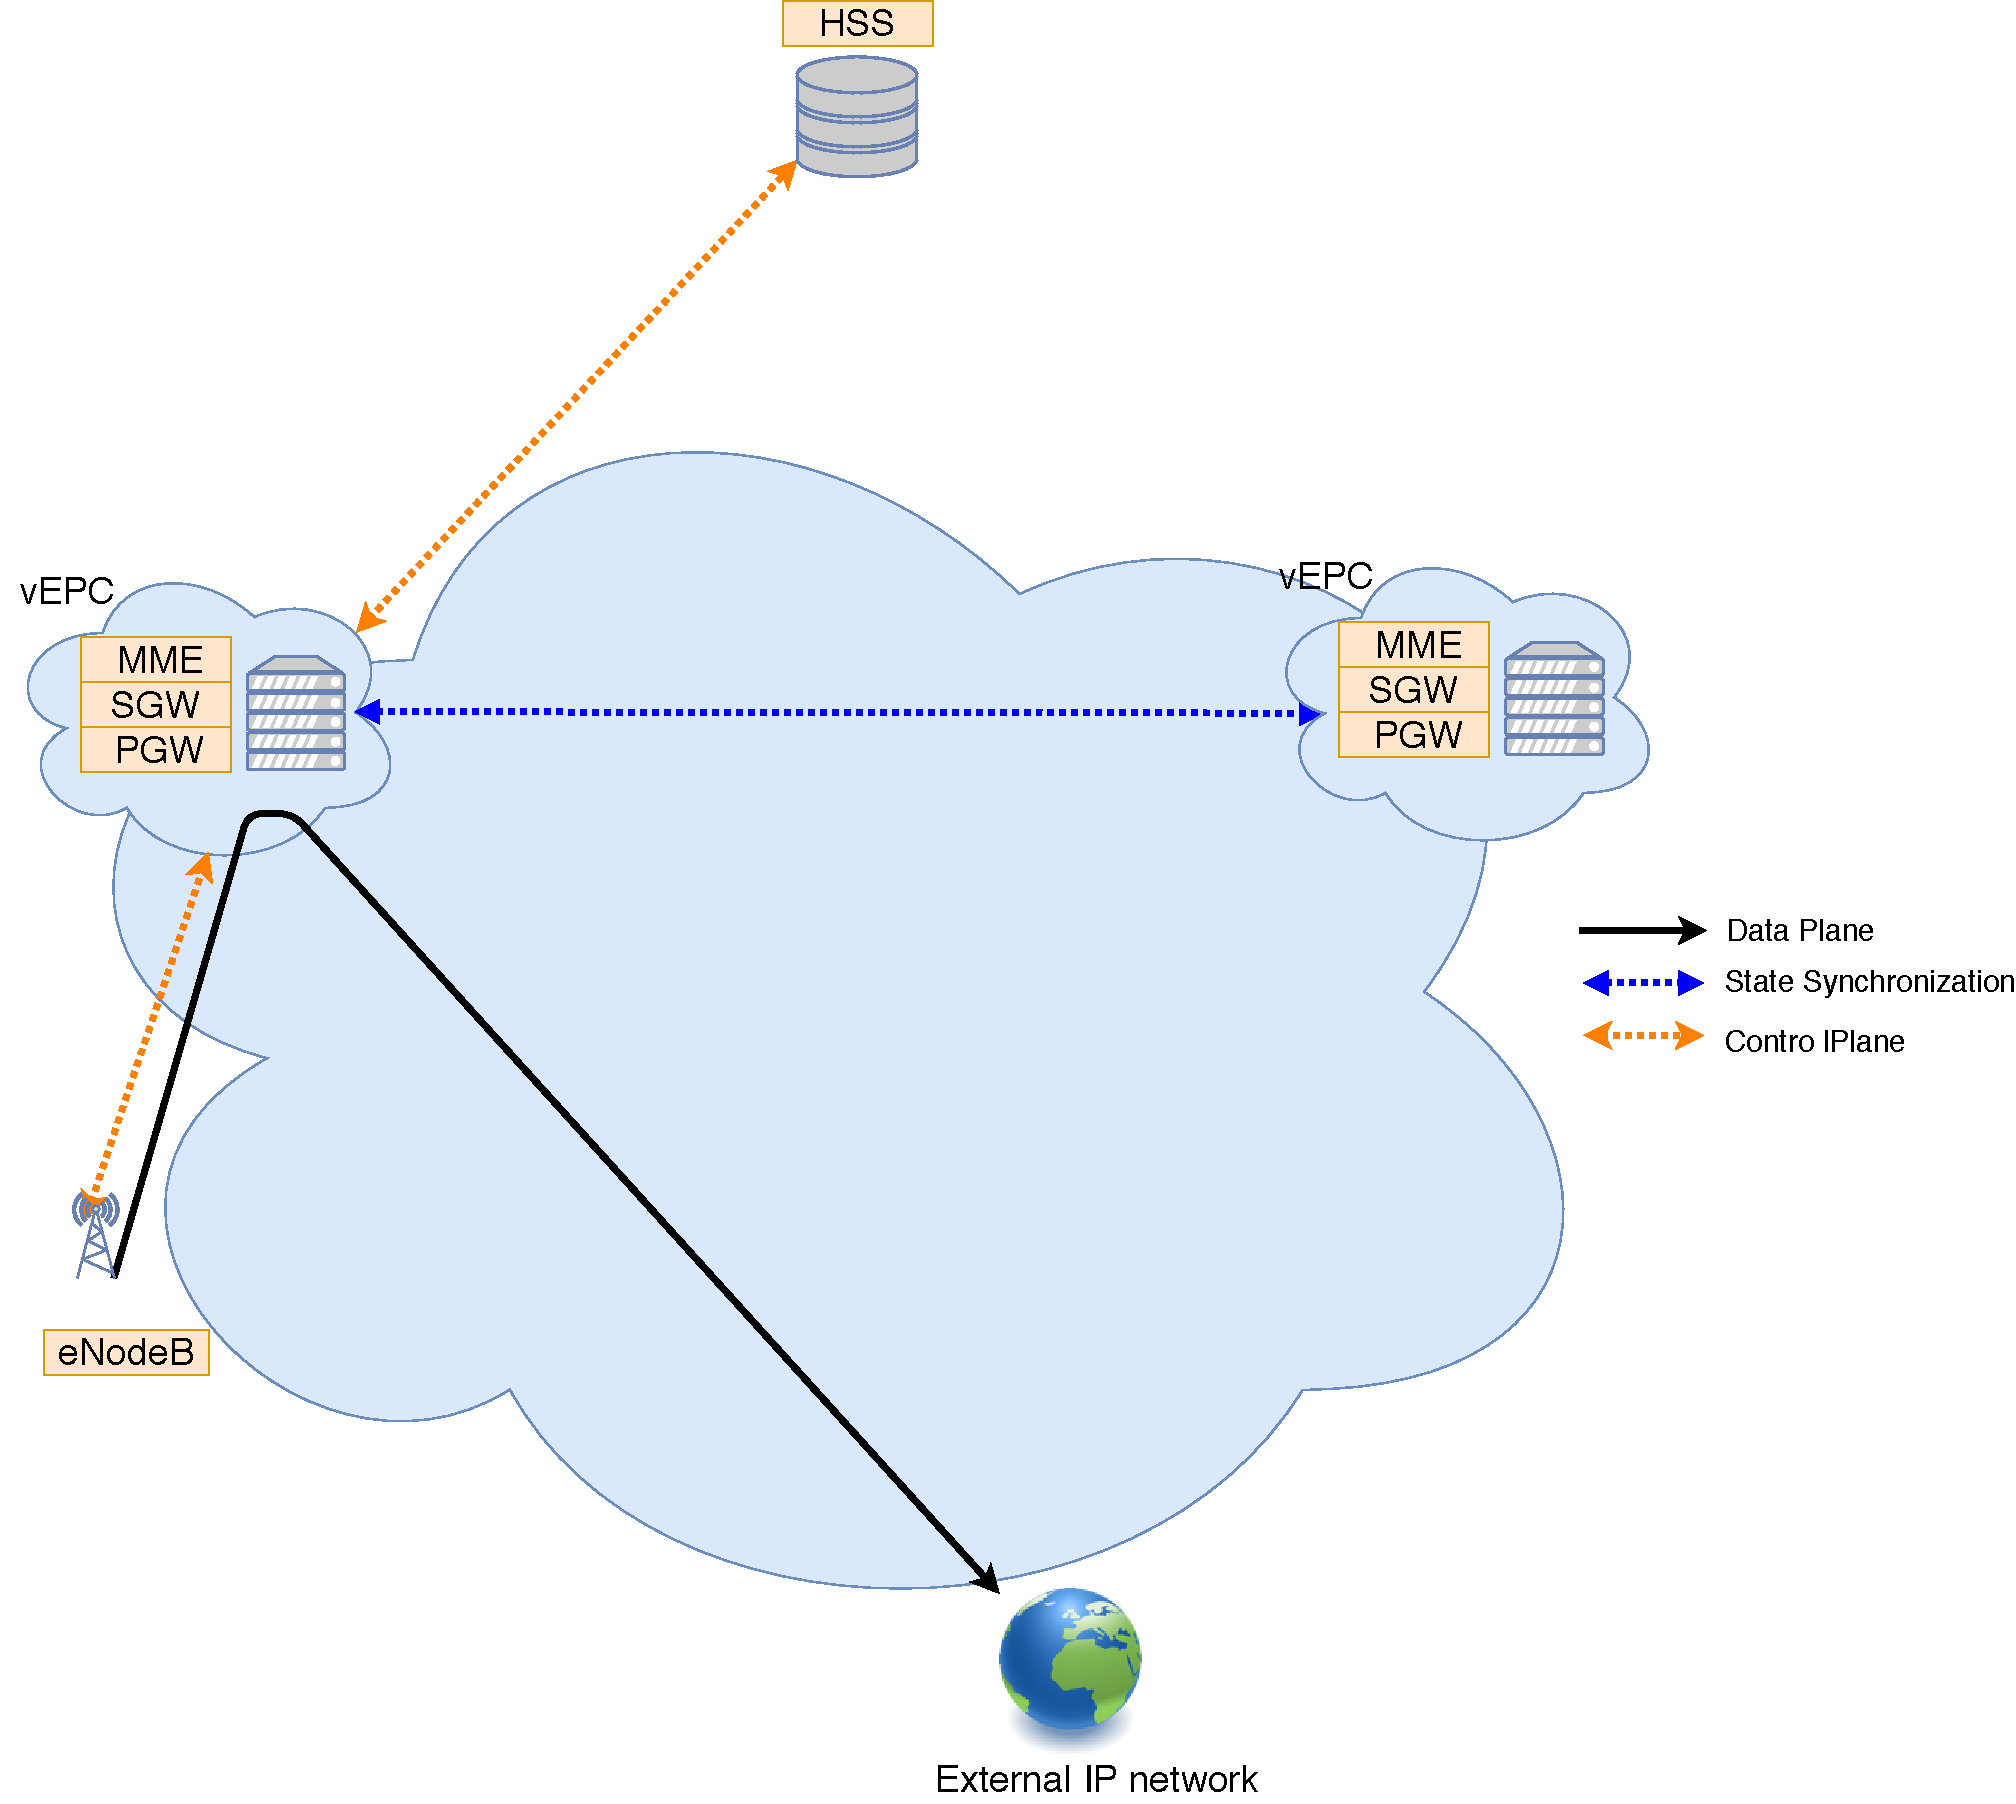
\includegraphics[width=0.5\hsize]{vEPC_before.pdf}
			\caption{before}
			\label{vEPC_before}
		\end{subfigure}
		\begin{subfigure}{1.0\textwidth}
		\centering
			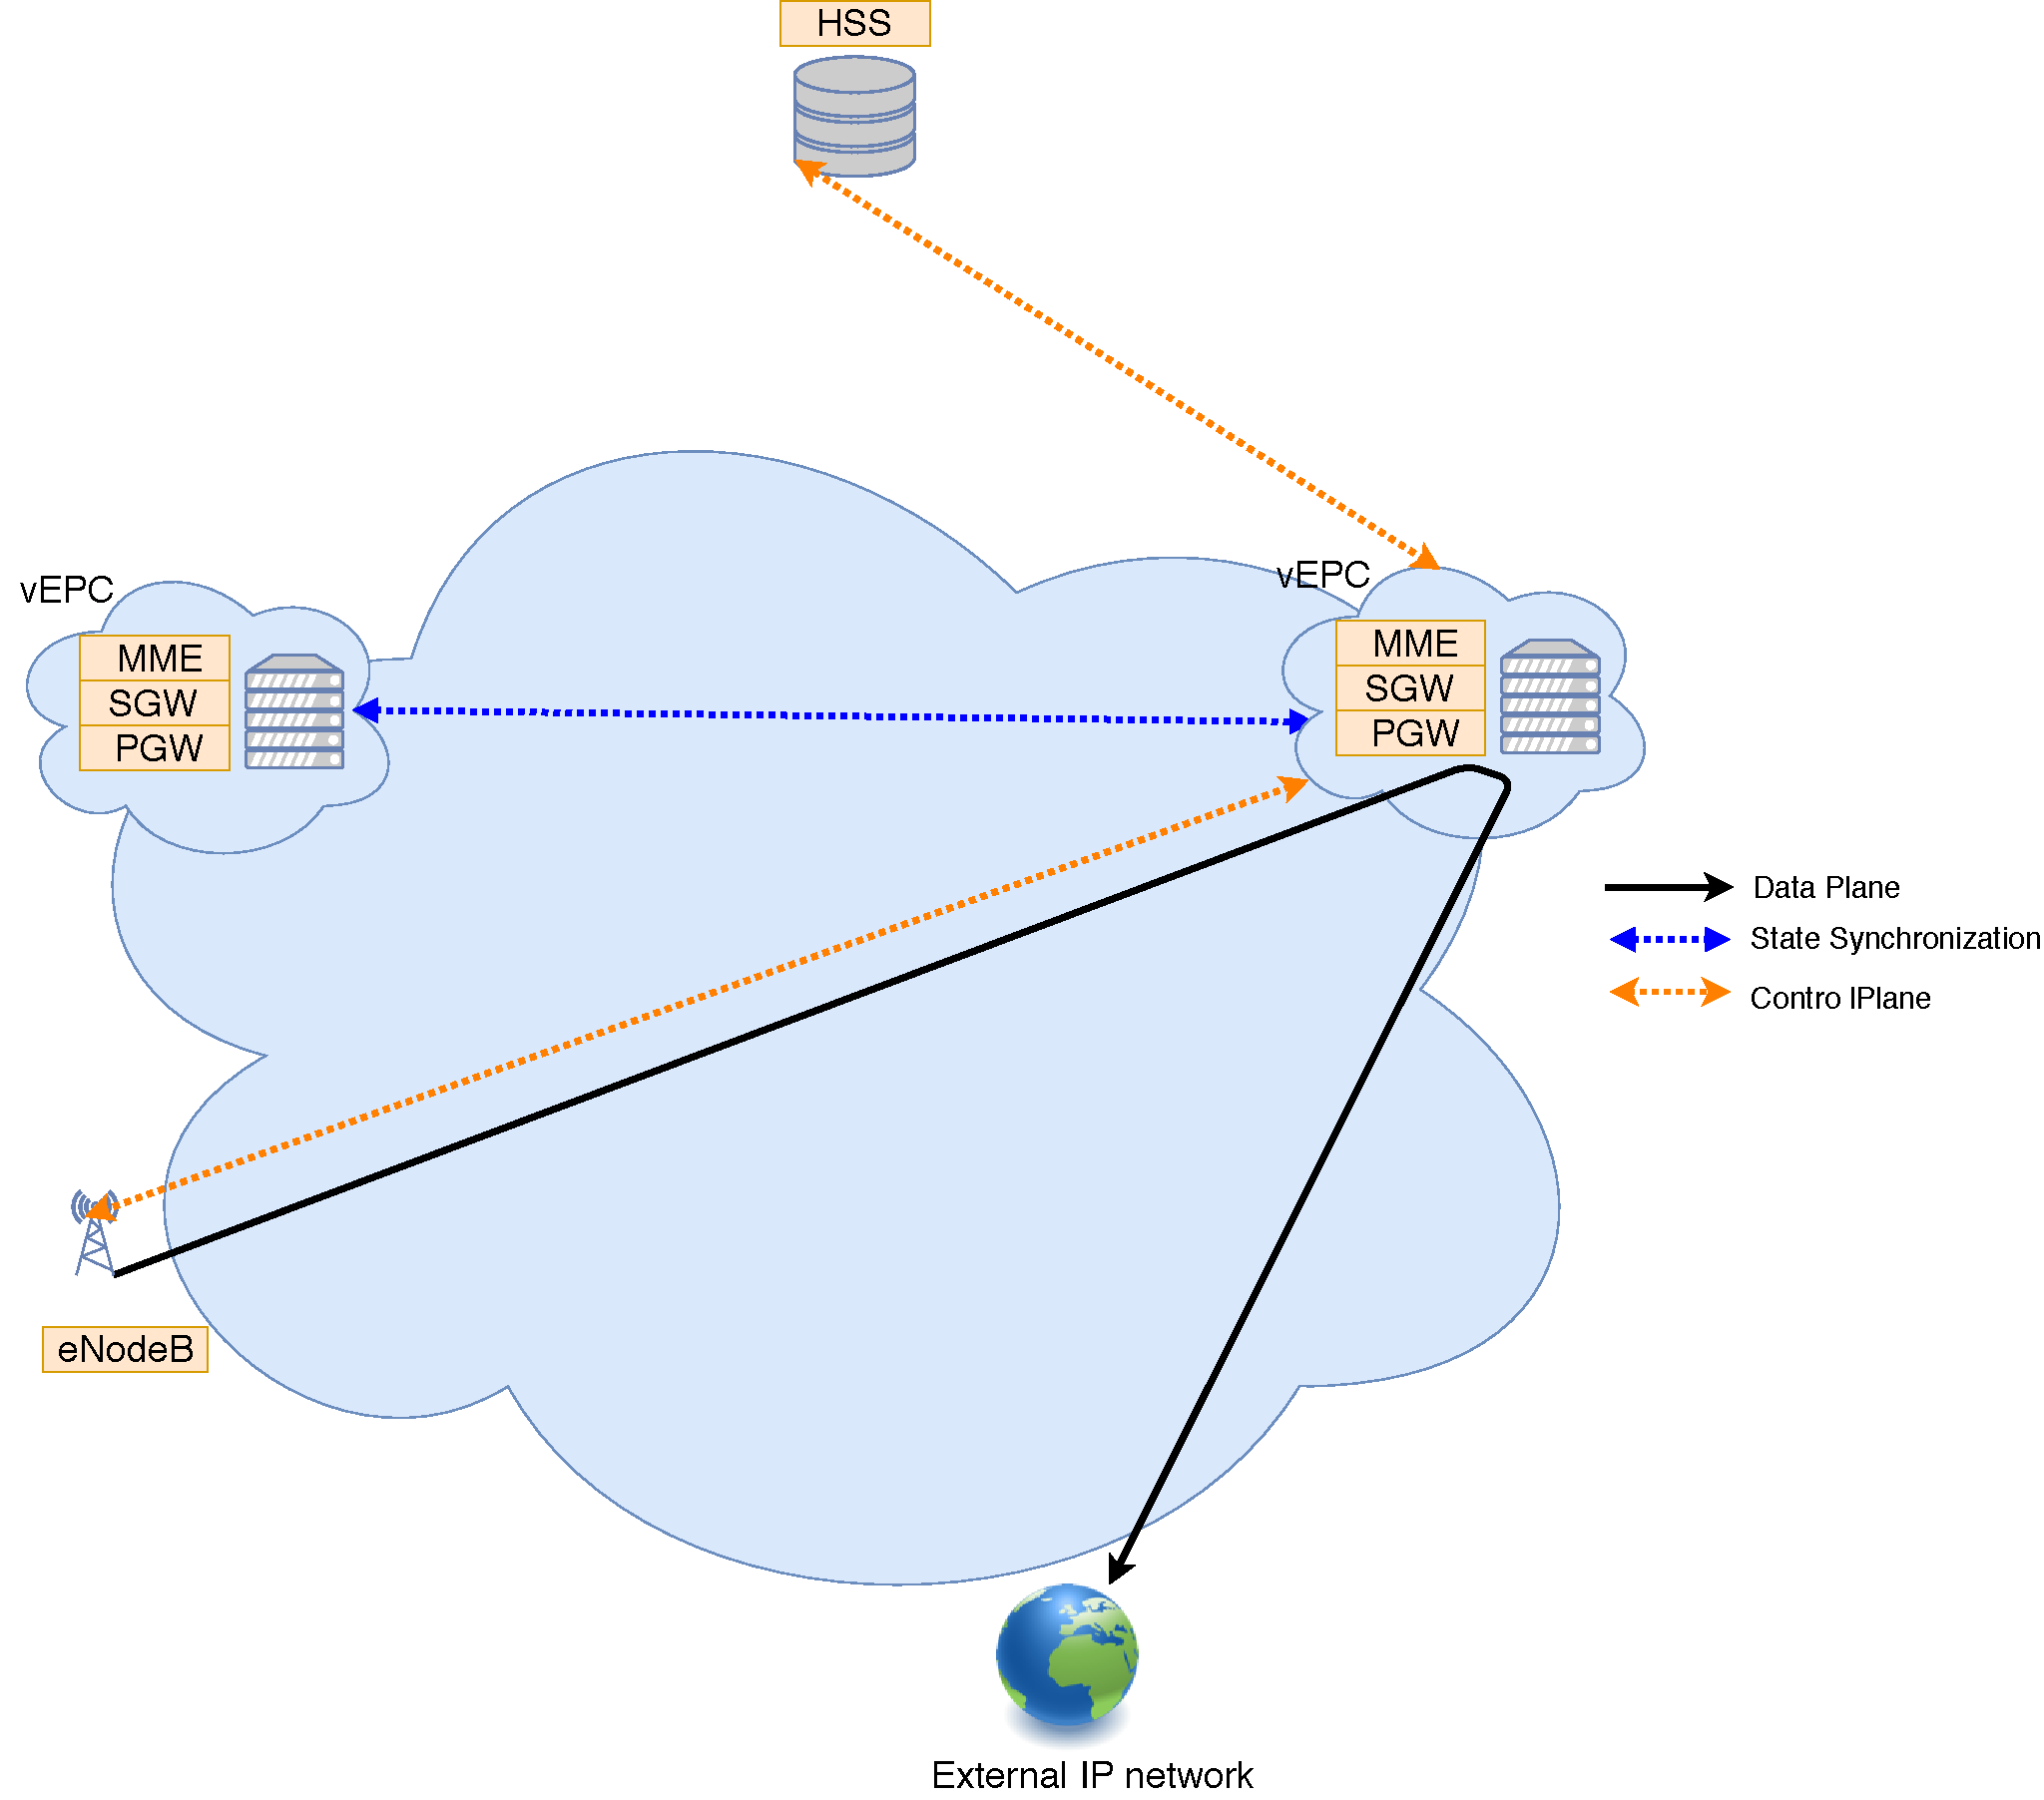
\includegraphics[width=0.5\hsize]{vEPC_after.pdf}
			\caption{after}
			\label{vEPC_after}
		\end{subfigure}
		\caption{vEPCを想定したネットワークモデル(案)}
		\label{vEPC}
\end{figure}

\begin{figure}[p]
	\centering
		\begin{subfigure}{1.0\textwidth}
		\centering
			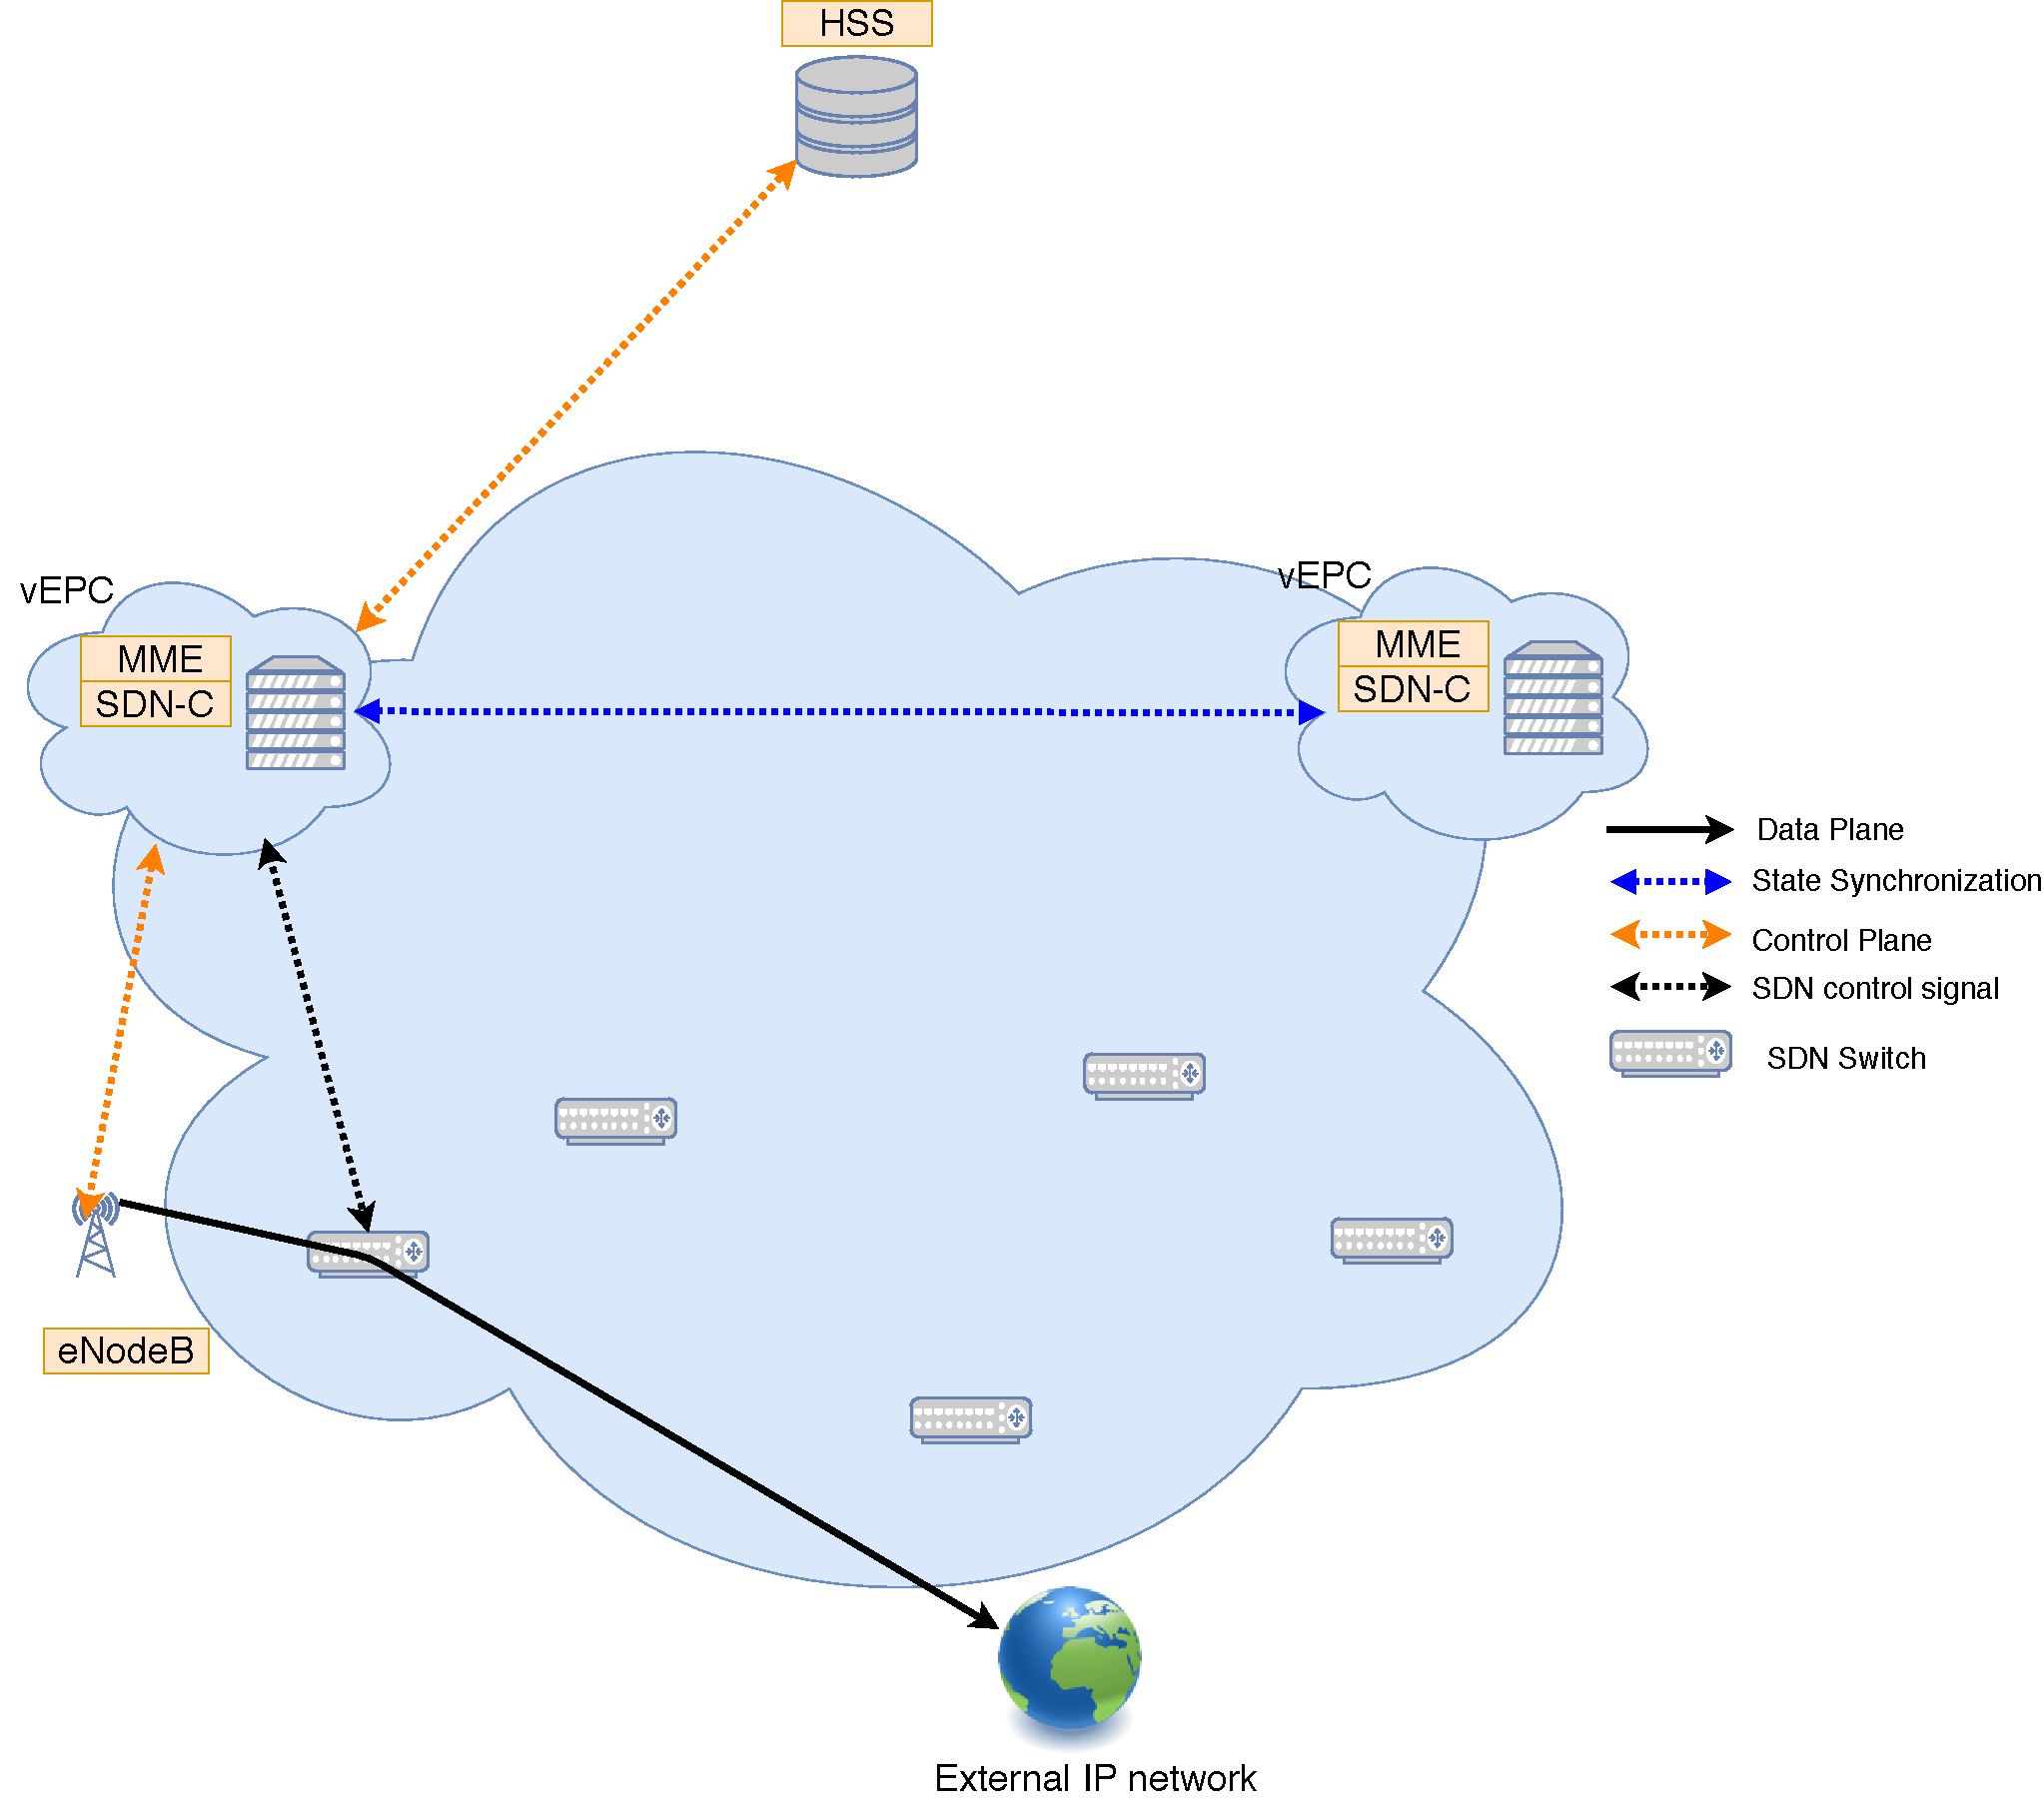
\includegraphics[width=0.5\hsize]{vEPC_SDN_before.pdf}
			\caption{before}
			\label{vEPC_SDN_before}
		\end{subfigure}
		\begin{subfigure}{1.0\textwidth}
		\centering
			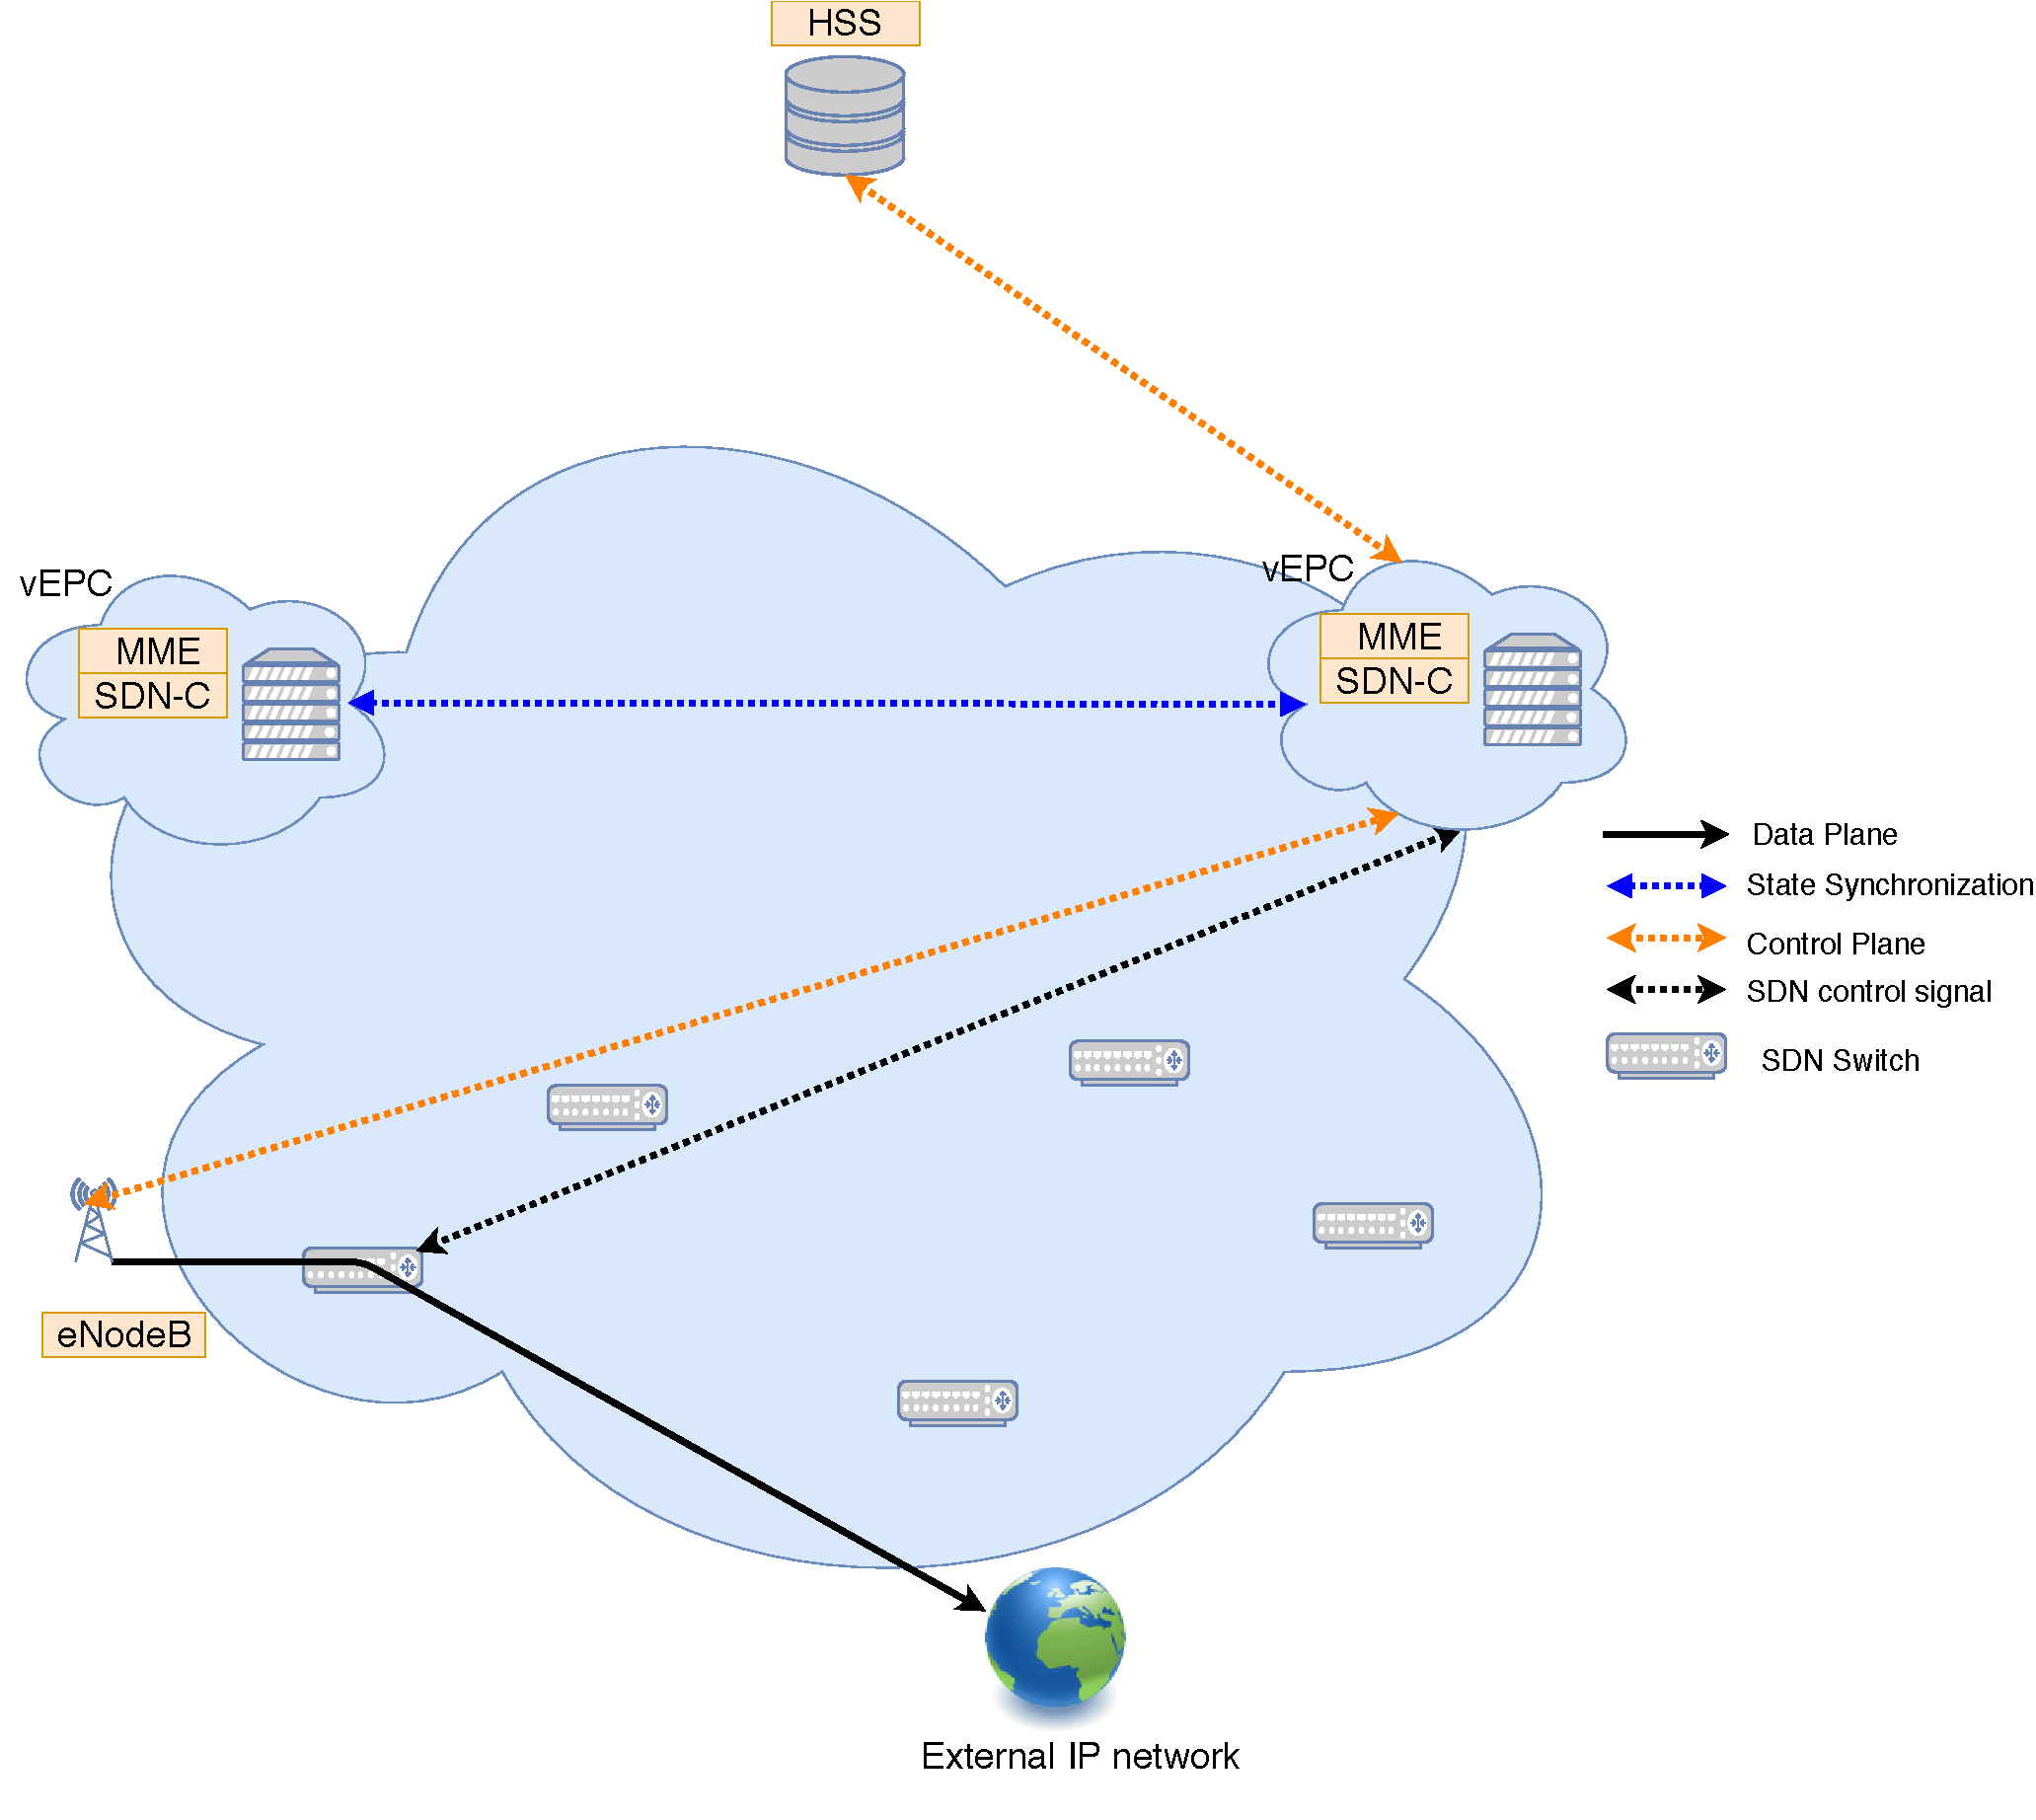
\includegraphics[width=0.5\hsize]{vEPC_SDN_after.pdf}
			\caption{after}
			\label{vEPC_SDN_after}
		\end{subfigure}
		\caption{vEPCを想定したネットワークモデル(案2)}
		\label{vEPC_SDN}
\end{figure}

% \begin{figure}[htbp]
% 	\centering
% 	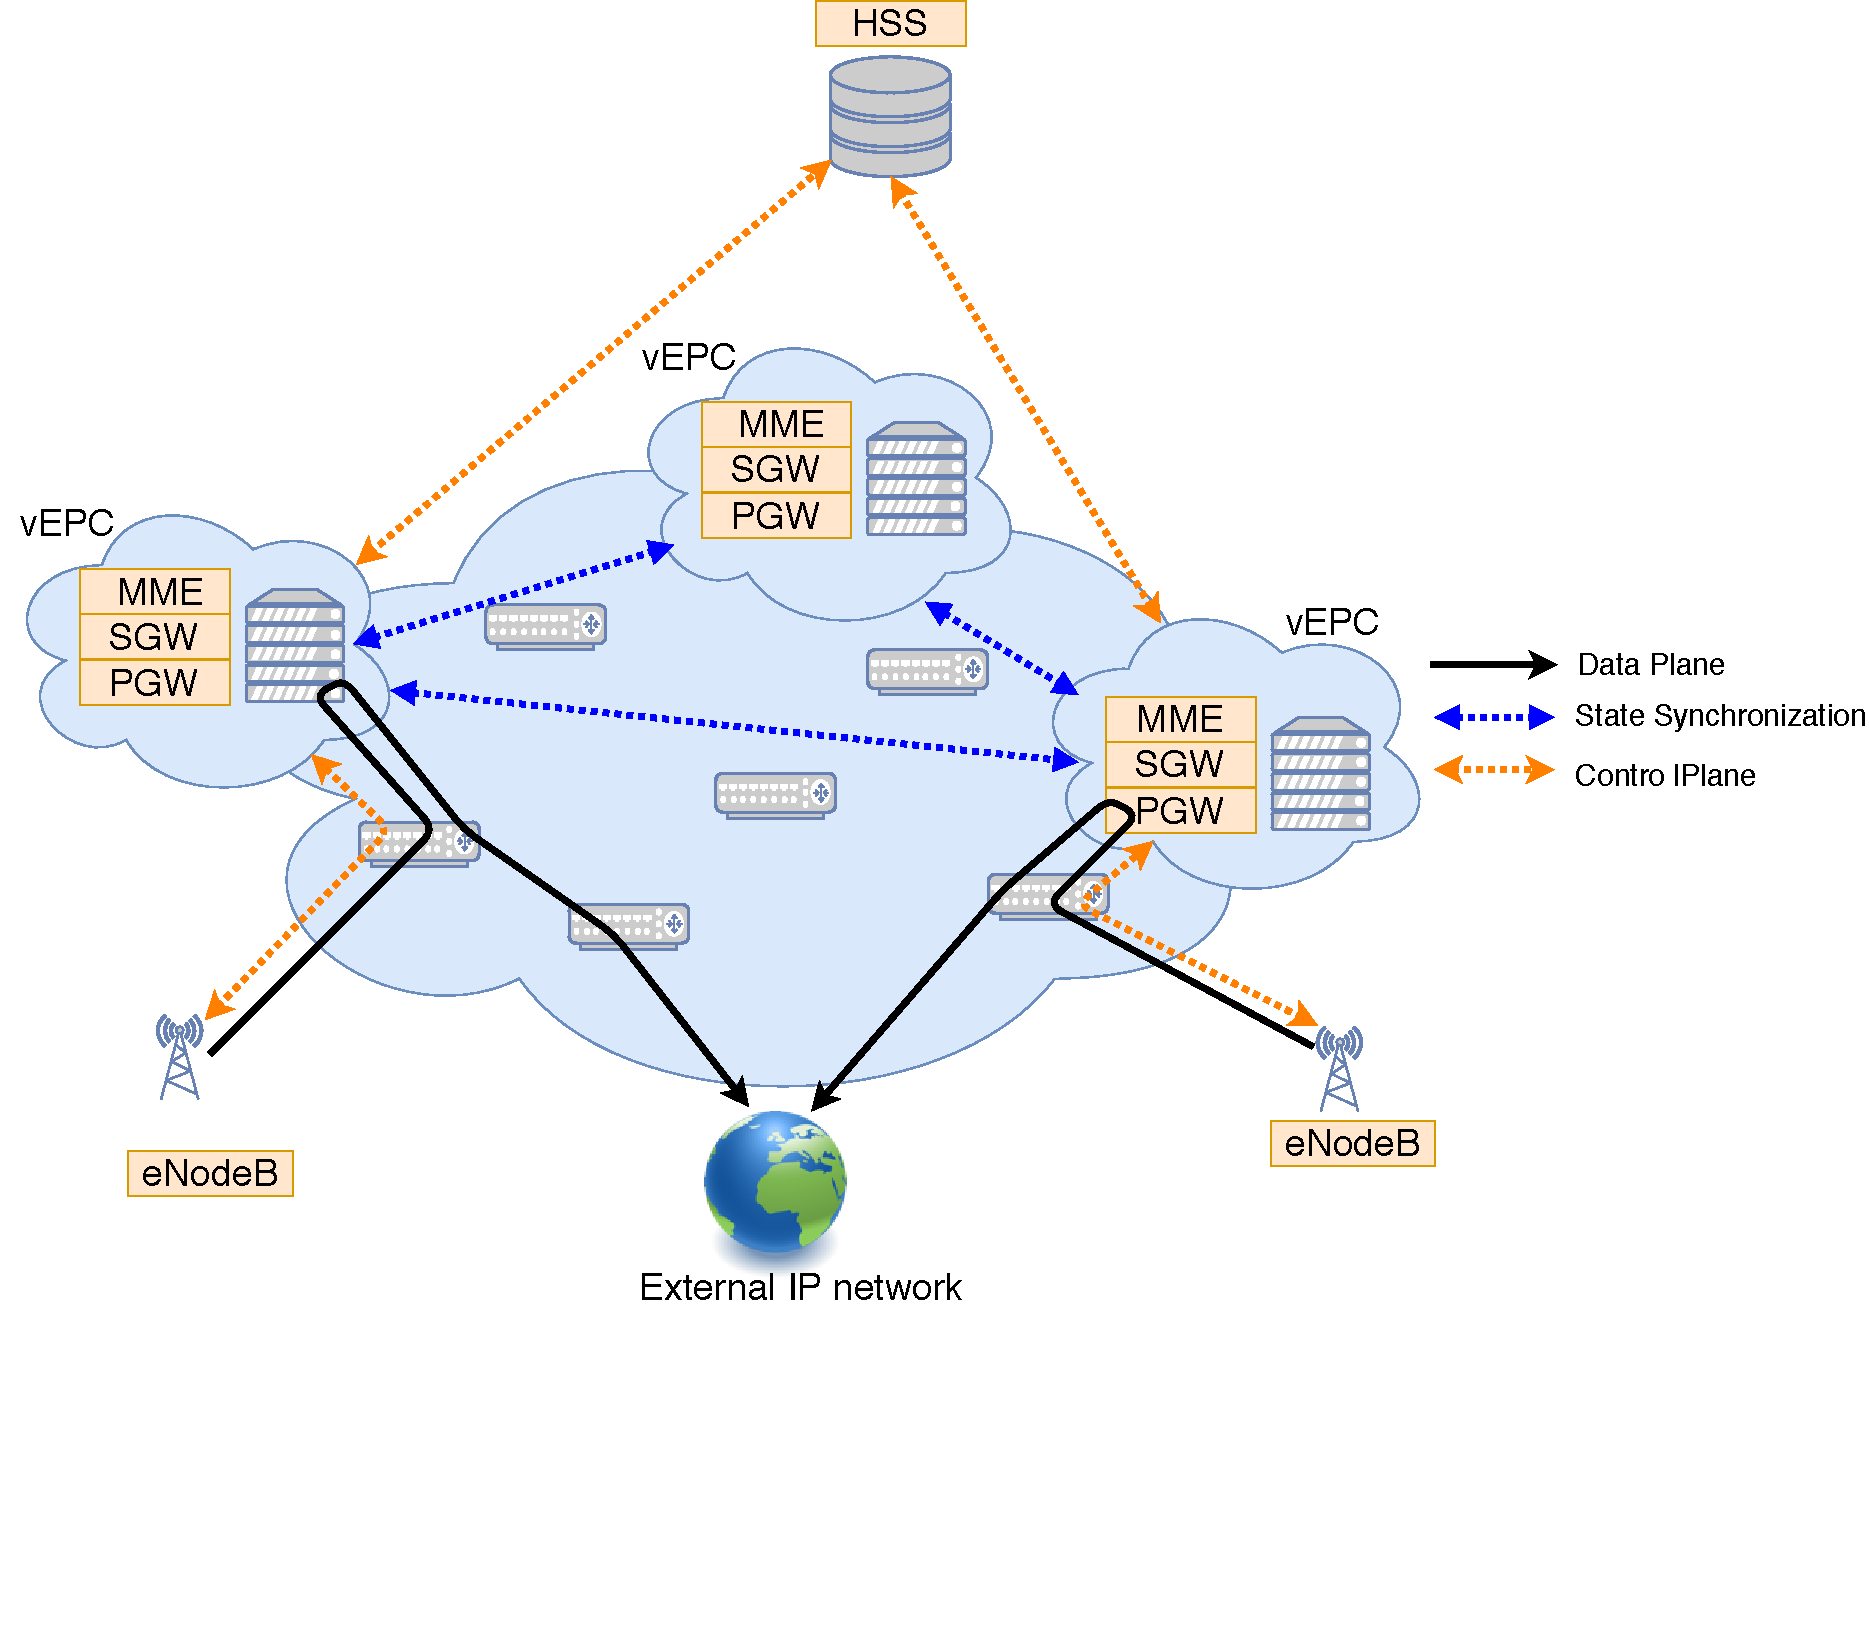
\includegraphics[width=0.7\hsize]{vEPC_model.pdf}
%   \caption{vEPCを想定したネットワークモデル(案)}
% 	\label{vEPC_model}
% \end{figure}
%
% \begin{figure}[htbp]
% 	\centering
% 	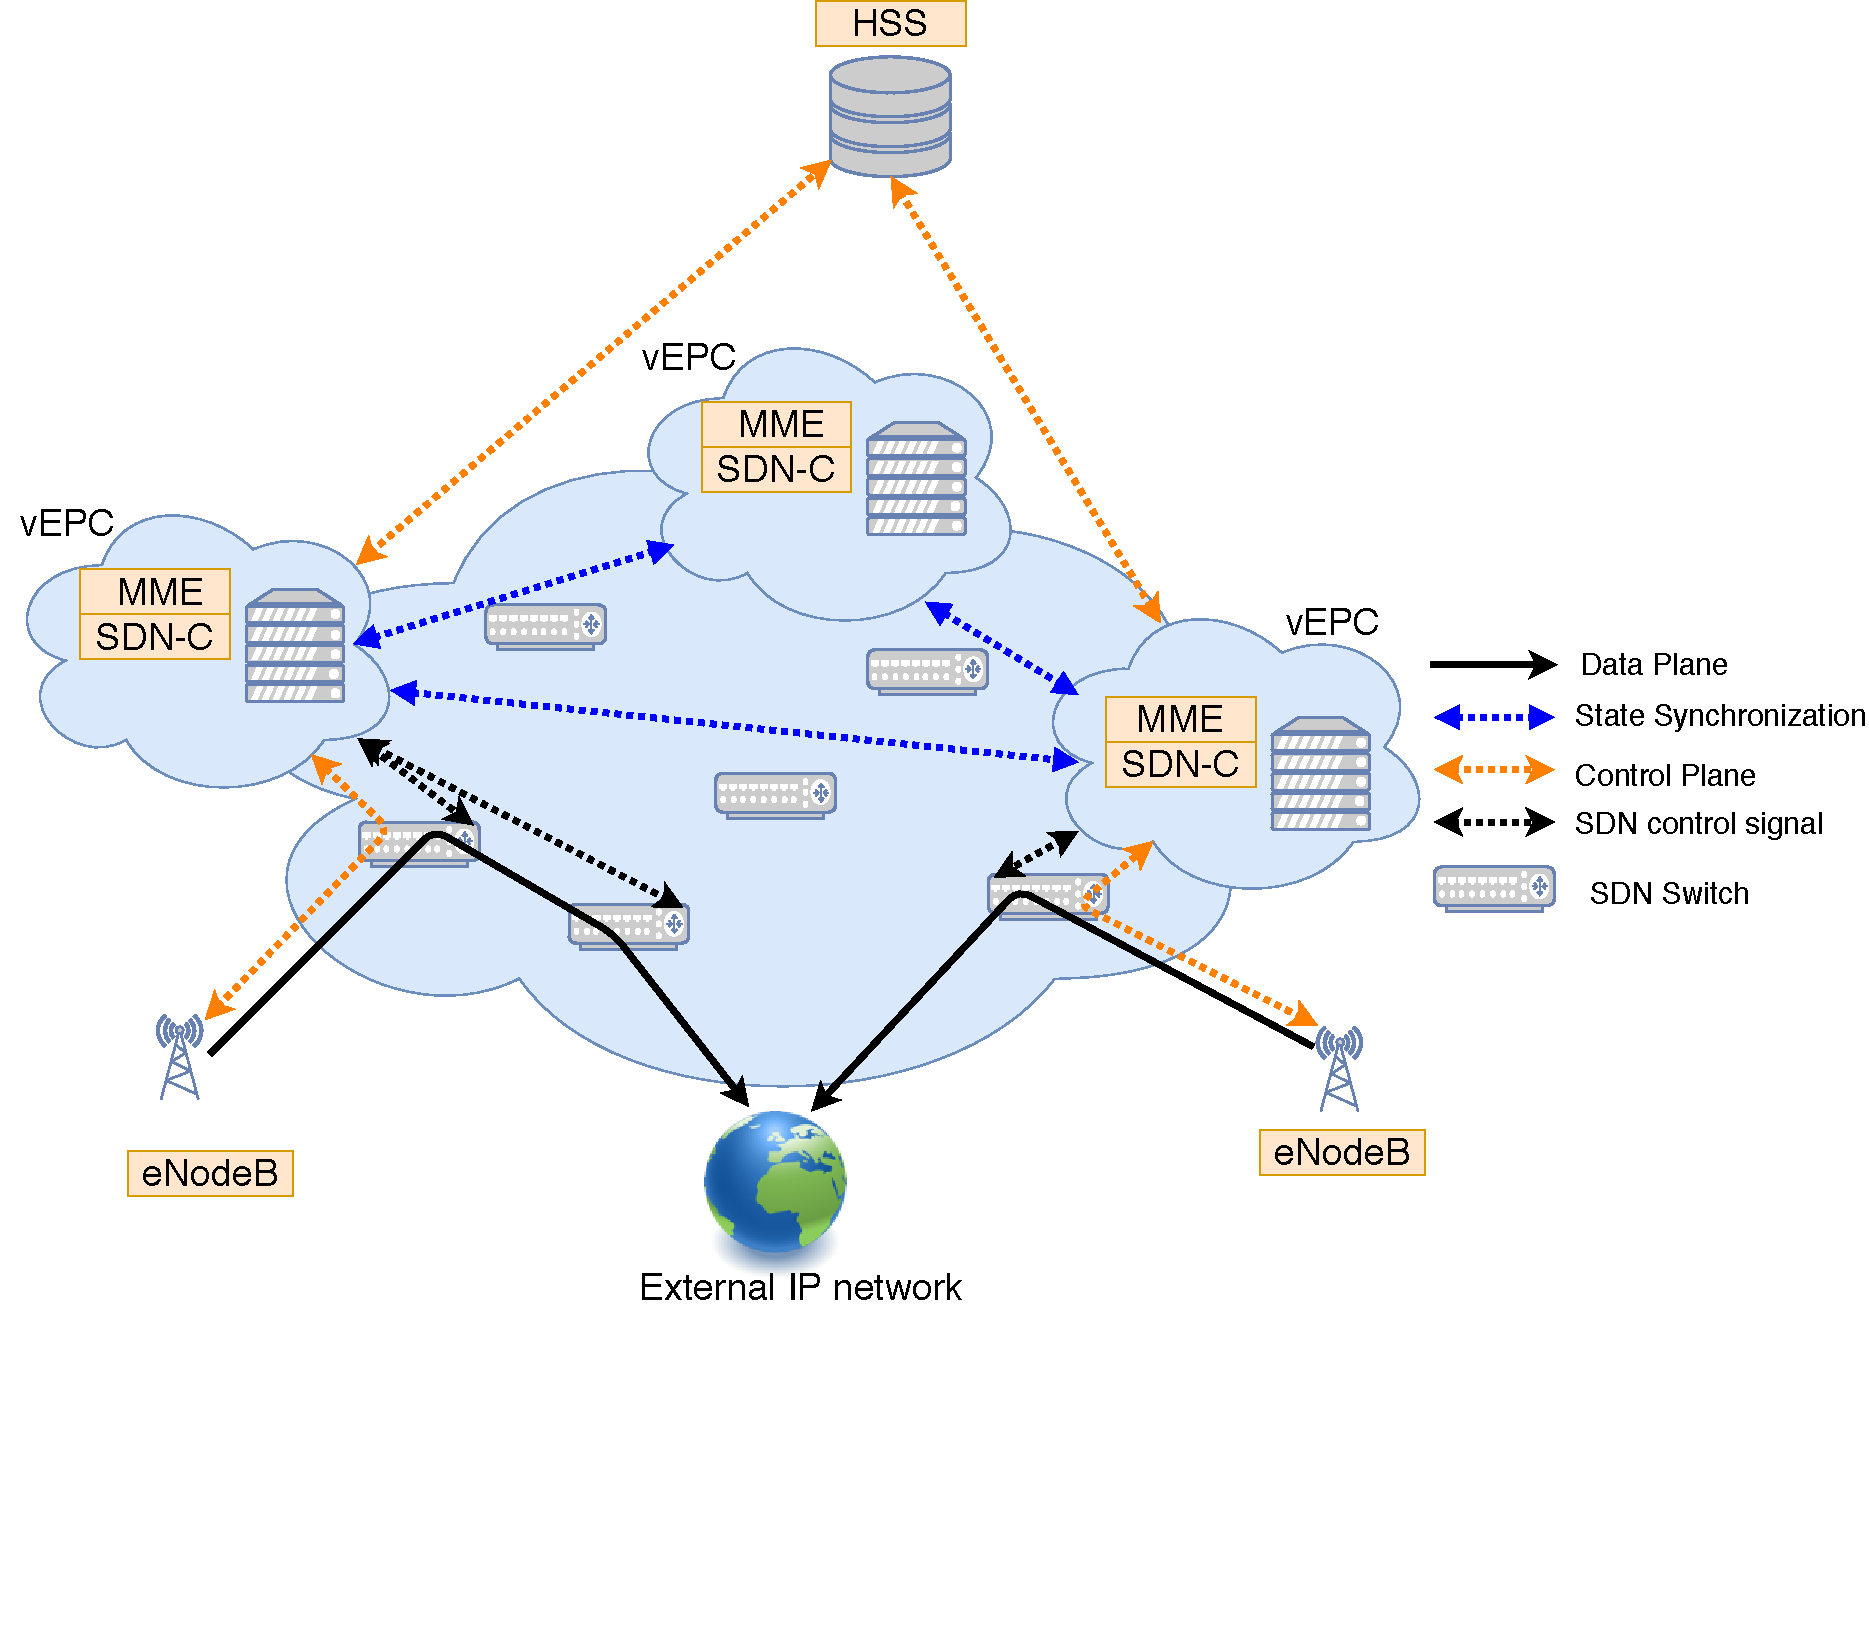
\includegraphics[width=0.7\hsize]{vEPC_SDN_model.pdf}
%   \caption{vEPCを想定したネットワークモデル(案2)}
% 	\label{vEPC_SDN_model}
% \end{figure}

\clearpage


\section{ステート同期について}
\subsection{頻度}
ステート同期の頻度として、シグナリングメッセージ単位で行う方法と、セッション単位で行う方法がある。シグナリングメッセージ単位の方法では、よりきめ細かい同期が可能となる。しかし、私の評価では、vEPCの切り替えはシグナリング単位ではなくセッション単位で行うことを想定している。つまり、アタッチなどの処理は、その一連の処理がするまで同一のvEPCで管理される。そのため、ステート同期の頻度はセッション単位で十分であり、研究としてはセッション単位のステート同期をメインに評価するつもりである(比較としてシグナリングメッセージ単位の同期を考える可能性がある)。
\subsection{負荷}
待ち行列を用いた数学的評価によってステート同期の影響を評価する。そのためには、EPCノードの負荷をコード行数から推定したのと同じように、ステート同期にかかる時間を何らかの指標から推定し、最終的に待ち行列理論に落とし込む必要がある。ステート同期は主に、データの読み書きであるため、I/O待ち時間に基づいた待ち行列理論によって、ステート同期のオーバヘッドを求める。

文献\cite{PerformanceComparisonofStateSynchronizationTechniquesinaDistributedLTEEPC}などの先行研究より、ステート同期によって発生するオーバーヘッドの大きさについてある程度、見当をつけることができる。そのような先行研究を参考にしつつ、I/O待ち時間をパラメータとして変化させ、それぞれの場合について評価することも想定している


\section{勉強会論文まとめ}
勉強会で調査した論文を以下の表\ref{matome}にまとめる。

\begin{landscape}

\begin{table}[htbp]
	{\scriptsize
	\centering
	\caption{論文まとめ}
	\label{matome}
  \begin{tabular}{c||c|cc|ccc|c|c}\hline
    \multicolumn{1}{c||}{References}&\multicolumn{1}{c|}{Technology}&\multicolumn{2}{c|}{Routing}&\multicolumn{3}{c|}{Load Balancing}&\multicolumn{1}{c|}{Eval.}&\multicolumn{1}{c}{Key Word}\\ \cline{3-7}
		&&GTP&Non-GTP&SGW&PGW&MME&Methods\\ \hline\hline
		\cite{EfficientExploitationofMobileEdgeComputingforVirtualized5GinEPCArchitectures}&NFV&\Checkmark&-&\Checkmark&\Checkmark&\Checkmark&Exptl.&MEC \\ \hline
		\cite{PerformanceComparisonofStateSynchronizationTechniquesinaDistributedLTEEPC}&-&-&-&\Checkmark&\Checkmark&\Checkmark&Exptl.&LoadBalancer\\ \hline
    \cite{VirtualMobileCorePlacementforMetroNetwork}&NFV+Chaine&-&\Checkmark&\Checkmark&\Checkmark&\Checkmark&Simul.&Service Chains\\ \hline
    \cite{NovelLIPASIPTOOffloadingAlgorithmAccordingtotheNetworkUtilizationandOffloadingpPreference}&LIPA/SIPTO&-&-&\Checkmark&\Checkmark&\Checkmark&Simul.&LIPA/SIPTO\\ \hline
		\cite{AcloudnativesolutionfordynamicautoscalingofMMEinLTE}&NFV&-&-&-&-&\Checkmark&Exptl.&CNS-MME  \\ \hline
		\cite{AnalyticalmodelingforVirtualizedNetworkFunctions}&NFV&\Checkmark&-&-&-&\Checkmark&Analy.\&Simul.&待ち行列を用いた負荷分散の性能評価 \\ \hline
		\cite{NetworkOrchestrationforDynamicNetworkSlicingforFixedandMobileVerticalServices}&SDN&-&-&\Checkmark&\Checkmark&-&Exptl.&MPLS, T-SDN  \\ \hline
    \cite{AnAdaptiveMechanismforLTEPGWVirtualizationUsingSDNandNFV}&SDN+NFV&-&\Checkmark&-&\Checkmark&-&Exptl.&SDMN \\ \hline
		\cite{AnInnovativeEPCwithNotOnlyStackforbeyond5GMobileNetworks}&SDN+NFV&\Checkmark&-&-&-&-&Simul.&NOS-EPCの提案、評価 \\ \hline
		\cite{VirtualisingandOrchestratinga5GEvolvedPacketCoreNetwork}&SDN+NFV&\Checkmark&-&-&-&-&Exptl.&VM実装と実マシン実装の性能比較 \\ \hline
		\cite{Software-DefinedControloftheVirtualizedMobilePacketCore}&SDN+NFV&\Checkmark&-&-&-&-&-&MEC \\ \hline
		\cite{IntegratedSDN/NFVOrchestrationfortheDynamicDeploymentofMobileVirtualBackhaulNetworksOveraMultilayer(packet/optical)AggregationInfrastructure}&SDN+NFV&-&-&-&-&-&Exptl.&vEPC, vSDN \\ \hline
		\cite{NetworkServiceChaininginFogandCloudComputingforthe5GEnvironment:DataManagementandSecurityChallenges}&SDN+NFV&-&-&-&-&-&Simul.&MEC, セキュリティ対策 \\ \hline
		\cite{NetworkSlicingfor5GwithSDNNFVConceptsArchitecturesandChallenges}&SDN+NFV&-&-&-&-&-&-&Slicing \\ \hline
		\cite{AComparisonofSDNandNFVforRedesigningtheLTEPacketCore}&SDN+NFV&\Checkmark&-&-&-&-&Exptl.&OpenSourceを用いたNFV、SDNの実装 \\ \hline
		\cite{TowardsaCostOptimalDesignfora5GMobileCoreNetworkBasedonSDNandNFV}&SDN+NFV&-&-&-&-&-&Simul.&NFVとSDNの性能比較\\ \hline
	 	\cite{CostModelingforSDN/NFVBasedMobile5GNetworks}&SDN+NFV&-&-&-&-&-&Analy.&CAPEX、OPEXの評価モデル\\ \hline
 		\cite{ProposalandEvaluationofSDN‐basedMobilePacketCoreNetworks}&SDN&-&\Checkmark&-&-&-&Analy.&Openflow-enabled EPC \\ \hline
		\cite{SlicingVirtualizedEPCbased5GCoreNetworkforContentDelivery}&NFV&-&-&-&-&-&Analy.&CDN \\ \hline
		\cite{Signalingisgrowing50fasterthandatatraffic}&-&-&-&-&-&-&-&トラヒック量の統計\\ \hline
		\cite{ASDNBasedDistributedMobilityManagementinLTEEPCNetwork}&SDN&-&\Checkmark&-&-&-&Simul.&SDN-based distributed mobility management\\ \hline
		\cite{OptimizingServiceReplicationforMobileDelaySensitiveApplicationsin5GEdgeNetwork}&-&-&-&-&-&-&Analy.&MEC\\ \hline
		\cite{IoTTrafficModelsfor5GResearches}&-&-&-&-&-&-&-&IoTトラヒックモデルの調査\\ \hline
		\cite{PerformanceEvaluationofOpen5GCoreoverKVMandDockerbyUsingOpen5GMTC}&NFV&-&-&-&-&-&Exptl.&Docker、KVM、実マシンでのOpen5GCoreの性能比較\\ \hline
		\cite{PerformanceAnalysisofVNFsforSizingCloudRANInfrastructures}&-&-&-&-&-&-&Simul.&C-RAN、BBU\\ \hline
		\cite{UnderstandingtheBottlenecksinVirtualizingCellularCoreNetworkFunctions}&-&-&\Checkmark&-&-&-&Analy.&待ち行列を用いたEPCのボトルネック調査\\ \hline
		\cite{Beta/M/1ModelforMachineTypeCommunication}&-&-&-&-&-&-&-&Beta分布を用いたコアネットワーク内の遅延評価\\ \hline
		\cite{OptimizedLTEDataTransmissionProceduresforIoTDeviceSideEnergyConsumptionAnalysis}&-&-&\Checkmark&-&-&-&-&マルコフ連鎖を用いたUEの消費電力モデルの策定\\ \hline
    \cite{OnEvaluatingDifferentTrendsforVirtualizedandSDNReadyMobileNetwork}&SDN&\Checkmark&-&-&-&-&Exptl.&S/PGWのC/U分離とSDNの実装\\ \hline
		\cite{AssessmentofLTEWirelessAccessforMonitoringofEnergyDistributionintheSmartGrid}&-&-&-&-&-&-&Analy.&マルコフ連鎖を用いた無線通信のモデル化\\ \hline
		\cite{AnEmpiricalCaseforContainerDrivenFineGrainedVNFResourceFlexing}&-&-&-&-&-&-&Exptl.&BareMetal、Docker、VMの性能比較\\ \hline
		\cite{SoftwareDefinedNetworkingtoSupportIPAddressMobilityinFutureLTENetwork}&SDN&\Checkmark&-&\Checkmark&\Checkmark&-&Simul.&SDNを用いたS/PGWの分散配置\\ \hline
		自分の研究&SDN&\Checkmark&-&\Checkmark&\Checkmark&\Checkmark&Analy.\\ \hline
	\end{tabular}
	}
\end{table}

\end{landscape}


\section{今後の予定}

\begin{itemize}
  \item I/O待ち時間の調査を行う。具体的には先行研究論文や富士通株式会社などが公開しているサーバパフォーマンスに関するホワイトペーパーなどを参考にする。
	% \item PCRFの配置および課金処理の実現方法についての調査。
\end{itemize}

\section*{\addcontentsline{toc}{section}{参考文献}}
{\scriptsize
\bibliographystyle{IEEEtran}
\bibliography{/Users/t-adachi/Documents/study/Bibliography/bib/hpt_core_network/myBib/LABbiblio,/Users/t-adachi/Documents/study/Bibliography/bib/hpt_core_network/Study_Group_Bibtex/bib/hptCoreNetwork_Study}
}
\end{document}
